%!TEX root = ../main.tex
% \begin{frame}{\emph{Smart} TVs}
%    \ \  \\[0.1cm]
%   \begin{itemize}
%   \item Capacidades interativas
%   \item Conexão à internet
%   \item Conteúdo de mídia transmitido a partir de outros dispostivo
% \end{itemize}
% \end{frame}
%
% \begin{frame}{\emph{Smart} TVs}
% \begin{figure}[h!]
% 	\includegraphics[width=0.6\textwidth]{img/smart_samsung.jpg}
% 	\caption{Diagrama representativo de uma \emph{Smart} TV e seus componentes}
% 	\label{fig:smart_samsung}
% \end{figure}
% \end{frame}
%
%
% \begin{frame}{\emph{Smart} TVs}
%   \begin{figure}[h!]
%   	\centering
%   	\includegraphics[width=0.6\linewidth]{img/sbt_app.jpg}
%   	\caption{Aplicativo SBT}
%   	\label{fig:sbt_app}
%   \end{figure}
% \end{frame}
%
% \begin{frame}{\emph{Smart} TVs}
%    \ \  \\[0.1cm]
%   \begin{itemize}
%   \item PNAD 2015
%   \begin{itemize}
%     \item $103$ milhões de aparelhos de televisões em residências e pontos comerciais
%     \item $16$ milhões de \emph{Smart} TVs
%     \item $94\%$ destas \emph{Smart} TVs foram adquiridas entre $2014$ e $2015$
%     \item $68,2\%$ do total de televisores vendidos no primeiro semestre de $2017$
%   \end{itemize}
% \end{itemize}
% \end{frame}
%
% \begin{frame}{\emph{Smart} TVs}
%    \ \  \\[0.1cm]
%   \begin{itemize}
%   \item Benefícios resultantes do uso de \emph{Smart}
%
%   \item Encerramento da transmissão de sinal analógico da televisão aberta
%   \item Copa do Mundo 2018
%   \item Tecnologia 4K
% \end{itemize}
% \end{frame}
%
% \begin{frame}{Classificação Indicativa}
%    \ \  \\[0.1cm]
%   \begin{itemize}
%   \item Sistema de garantias dos direitos da criança e do adolescente
%   \item Reserva-se o direito final aos pais e responsáveis
%   \item Órgão responsável: Cocind, vinculada ao Ministério da Justiça
%   \item Análise de classificação indicativa
%   \begin{itemize}
%     \item Grau de incidência de conteúdos impróprios
%   \end{itemize}
% \end{itemize}
% \end{frame}

\begin{frame}{\emph{Machine Learning}}
   \ \  \\[0.1cm]
  \begin{itemize}
  \item Estudo sistemático de algoritmos e sistemas que são capazes de melhorar seu desempenho com a experiência
  \ \ \newline
  \item \alert{Redes Neurais Artificiais}
  \begin{itemize}
  \item Cérebro humano
  \ \ \newline
  \item Neurônios: unidades de processamento simples
   \ \ \newline
  \item Capacidade de capturar tendências
   \ \ \newline
  \item Generalização
\end{itemize}
\end{itemize}
\end{frame}

\begin{frame}{Redes Neurais Artificiais}
   \ \  \\[0.1cm]
  \begin{itemize}
  \item McCulloch e Pitts, 1943
  \begin{figure}[ht]
  	\centering
  	\label{fig:neuronio}
  	\includegraphics[width=0.7\textwidth]{img/perceptron.png}
     \caption{Representação de um neurônio artificial}
  \end{figure}
\end{itemize}
\end{frame}

\begin{frame}{Redes Neurais Artificiais}
   \ \  \\[0.1cm]
   %!TEX root = ../main.tex

\begin{table}[H]
	\scalefont{0.8}
	\centering
	\label{tab:ativacoes}
	\begin{adjustbox}{width=0.7\textwidth}
		\begin{tabular}{l l p{6.5cm} l}
			\toprule
			Nome 			 		& Gráfico & Equação & Intervalo\\
			\midrule
			Identidade ou Linear		&
			 	\Centerstack{\includegraphics[width=0.15\textwidth]{img/identidade}}
			&
				$
					\begin{aligned}
						\sigma(z) = z
					\end{aligned}
				$
				& $(-\infty, + \infty) $\\
			\hline
			Tangente Hiperbólica		&
				\Centerstack{\includegraphics[width=0.15\textwidth]{img/tanh}}
				&
				$
					\begin{aligned}
						\sigma(z) = tanh(z) =\frac{(e^z - e^{-z})}{(e^z + e^{-z})}
					\end{aligned}
				$
				 & $(-1,1)$\\
			\hline
			Sigmoide ou Logística		&
				\Centerstack{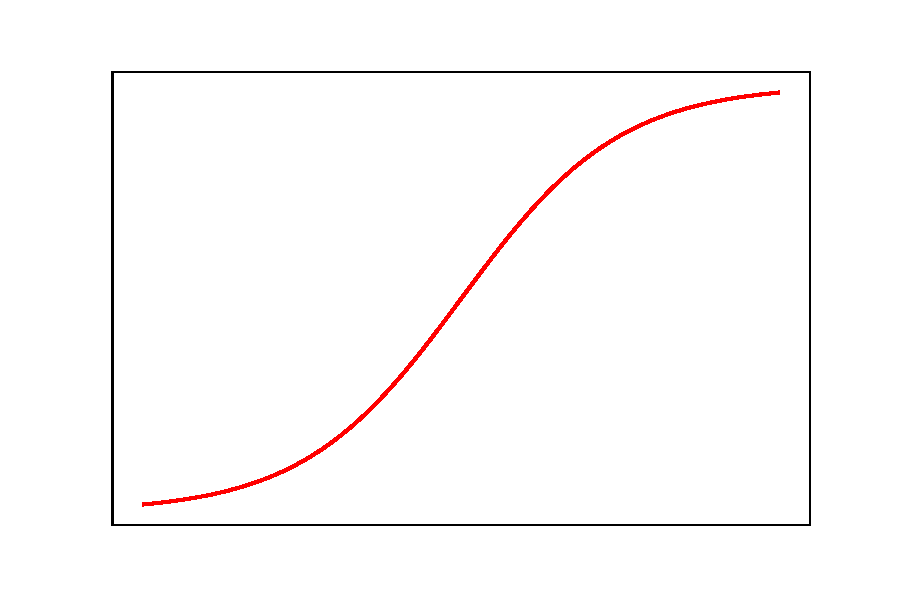
\includegraphics[width=0.15\textwidth]{img/sigmoid}}
				&
				$
					\begin{aligned}
						\sigma(z) = \frac{1}{1+e^{-x}}
					\end{aligned}
				$
				& $ (0,1) $\\
			\hline
			Unidade Linear Retificada	&
				\Centerstack{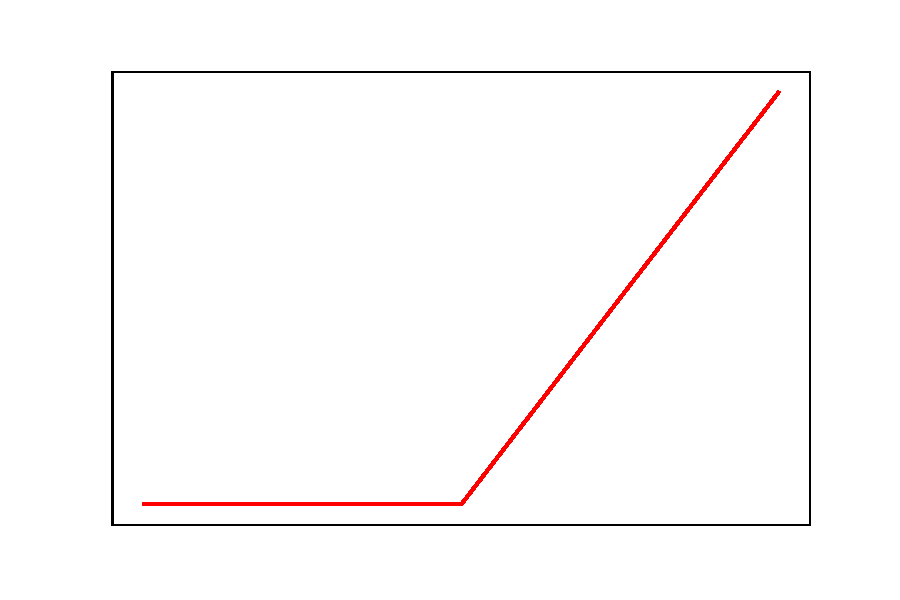
\includegraphics[width=0.15\textwidth]{img/relu}}
				&
				$
					\begin{aligned}
						\sigma(z) = max(0,z)
					\end{aligned}
				$
				& $ [0, \infty) $\\
			\hline
			Softmax					&
				\Centerstack{\includegraphics[width=0.15\textwidth]{img/softmax}}
				&
				$
					\begin{aligned}
						g(z_j) = \frac{e^{z_j}}{\sum^K_{j=1} e^{z_k}} \hspace{0.2cm}j=1, \ldots, K
					\end{aligned}
				$
				& $(-\infty, \infty)$\\
			\bottomrule
		\end{tabular}
	\end{adjustbox}
	\caption{Exemplos de funções de ativação}
\end{table}

\end{frame}

\begin{frame}{Redes Neurais Artificiais}
   \ \  \\[0.1cm]
  \begin{itemize}
  \item Perceptron de Rosenblatt (1958)
  \begin{itemize}
    \item Algoritmo de aprendizado
    \item Endereçava apenas problemas linearmente separáveis
  \end{itemize}
  \ \ \newline
  \pause
  \item Redes Neurais Artificiais
  \begin{itemize}
    \item Organização de múltiplos neurônios artificiais sob a forma de uma rede
    \item Resolução de problemas não-linearmente separáveis
  \end{itemize}
\end{itemize}
\end{frame}



\begin{frame}{Redes Neurais Artificiais}
   \ \  \\[0.1cm]
   \begin{itemize}
        \item Redes Neurais \alert{\emph{Multilayer Feedforward Perceptron}}
        \begin{itemize}
          \item Camada de entrada, camadas ocultas e camada de saída
          \item \emph{Feedforward} e completamente conectada
          \item Algoritmo \emph{Backpropagation}
          \begin{itemize}
               \item Fase \emph{forward}
               \item Fase \emph{backwards}
          \end{itemize}
\end{itemize}
   \end{itemize}
   \begin{figure}[ht]
    \centering
    \label{fig:mlp}
    \includegraphics[width=0.35\textwidth]{img/mlprna.jpg}
     \caption{Rede Neural MLP com duas camadas ocultas.}
   \end{figure}
\end{frame}

\begin{frame}{\emph{Deep Learning}}
   \ \  \\[0.1cm]
   \begin{itemize}
     \item Representar e reconhecer características sucessivamente complexas
     \ \ \newline
     \item Adição de níveis ou camadas de operações não-lineares
     \ \ \newline
     \item Resolver problemas complexos com um desempenho cada vez maior
     \begin{itemize}
       \item Aumento da quantidade de dados disponíveis
       \item Aumento do poder computacional
     \end{itemize}
     \ \ \newline
     \item \emph{ImageNet Large Scale Visual Recognition Challenge} (ILSVRC)
     \item $14$ milhões de imagens de $21$ mil categorias organizadas hierarquicamente
   \end{itemize}
\end{frame}

\begin{frame}{Redes Neurais Convolucionais}
   \ \  \\[0.1cm]
   \begin{itemize}
     \item Topologia bem definida e estrutura em grid
    \item Destaca-se no reconhecimento de padrões em dados de alta dimensionalidade
     \ \ \newline
     \item Diferentes tipos de camadas:
     \begin{itemize}
       \item Camada convolucional
       \item Camada de ativação
       \item Camada de pooling
     \end{itemize}

   \end{itemize}
\end{frame}

\begin{frame}{Redes Neurais Convolucionais}
   \ \  \\[0.1cm]
   \begin{itemize}
     \item Convolução
     \begin{equation}
      S(i,j) = I(i,j)*K(i,j) = \sum_{m}\sum_{n}I(m,n)K(i-m,j-n)\label{eq:conv_img}
     \end{equation}
   \end{itemize}
   \begin{figure}[!h]
   	\centering
   	\label{fig:convolutions}
   	\includegraphics[width=0.8\textwidth]{./img/fundamenta/convolutions}
     \caption{Papel das camadas convolucionais e \emph{feature maps} nas CNNs.}
   \end{figure}
\end{frame}

\begin{frame}{\LARGE{Modelos Canônicos de Redes Neurais Convolucionais}}
   \ \  \\[0.1cm]
   \begin{itemize}
     \item Arquiteturas que trouxeram contribuições importantes
     \item Comuns ainda hoje no cenário de DL
     \ \ \newline
     \item LeNet (1998)
     \item AlexNet (2012)
     \item VGG (2014)
     \item Inception (2014)
     \item ResNet (2015)
     \ \ \newline
     \item \emph{Transfer Learning}: Aproveitamento de parâmetros treinados
   \end{itemize}
\end{frame}
